% This is LLNCS.DOC the documentation file of
% the LaTeX2e class from Springer-Verlag
% for Lecture Notes in Computer Science, version 2.4
\documentclass[10pt]{sigplanconf}

\usepackage{color}
\usepackage{graphicx}
\usepackage{listings, tikz, xcolor}
\usepackage{bold-extra}
\usepackage{subfig}
\usepackage{enumerate}
\usepackage{courier}
\usepackage{syntax}
\usepackage{amsmath}
\usepackage{tabularx, multirow}
%\usepackage{amsthm}
\usepackage{hyperref}
\usepackage{MnSymbol}

\definecolor{lightGrey}{rgb}{0.9, 0.9, 0.9}
\newcommand{\hilight}{\makebox[0pt][l]{\color{lightGrey}\rule[-0.45em]{0.9\linewidth}{1.5em}}}
\newtheorem{mydef}{Definition}
\DeclareCaptionType{copyrightbox}
%
\lstset{
	language = [AspectJ]Java,
  basicstyle=\sffamily\small,
  numbers=left,
	numberstyle=\tiny\color[rgb]{0.25,0.25,0.25},
	numberblanklines=false,
  firstnumber=auto,
	breaklines=true,
  tabsize=2,
	emph={aspect,declare, adapter, instance pointcut, instance, adaptee, adapts, select, UNTIL,pc, instanceType, exp, removeExp, composite, inter, union, .add , .remove, .add_after, .add_before, .remove_after, .remove_before},
	emphstyle=\textbf,
	escapechar={~},
	showstringspaces= false,
	%frame=single,
	captionpos = b,
	numberbychapter=false,
	breakatwhitespace = true,
	columns=fullflexible
	}
\lstset{prebreak=\raisebox{0ex}[0ex][0ex]{\ensuremath{\rhookswarrow}}} % requires \usepackage{MnSymbol}
%\lstset{postbreak=\raisebox{0ex}[0ex][0ex]{\ensuremath{\rcurvearrowse\space}}} % requires \usepackage{MnSymbol}

\usetikzlibrary{arrows,shapes.multipart,shapes.arrows,shapes.misc,calc,fit,shadows,positioning,patterns}

\newcommand\bh{\tikz[remember picture]
					\node (begin highlight) {};
			 }
  \newcommand\eh{\tikz[remember picture]
		 \node (end highlight) {};
		 \tikz[remember picture, overlay]
		 \draw[yellow,line width=10pt,opacity=0.3] (begin highlight) -- (end
			highlight);
		 }

\newcommand{\lstinlineabstract}[1]{\lstinline[emph={#1},emphstyle=\textit]~#1~}

\newcommand{\todok}[1]{\textcolor{red}{\textbf{#1}}}

\newcommand{\lstinln}[1]{\lstinline~#1~}
\begin{document}


\title{Instance Pointcuts}
\subtitle{Selecting Object Sets Based on Life-Cycle Phases}


\authorinfo{Kardelen Hatun}
{TRESE, University of Twente, 7500AE Enschede, The Netherlands}
{k.hatun@utwente.nl}

\authorinfo{Christoph Bockisch}
{TRESE, University of Twente, 7500AE Enschede, The Netherlands}
{c.m.bockisch@utwente.nl}

\authorinfo{Mehmet Aksit}
{TRESE, University of Twente, 7500AE Enschede, The Netherlands}
{m.aksit}


\maketitle

\begin{abstract}
In the life-cycle of objects there are different phases. The phase in which an object currently is, affects how it is handled in an application; however phase shifts are typically implicit.
In this study we propose an extension to the aspect-oriented language AspectJ with a new mechanism, called \emph{instance pointcuts}, for creating and maintaining categories of objects according to events in their life-cycle; these events are selected with pointcut-like specifications.


The selection criteria of instance pointcuts can be refined, e.g., by restricting the scope of an existing instance pointcut; and they can be composed, e.g., by boolean operations.
We offer a means to access all objects currently selected by an instance pointcut from Java code, i.e., to be used in methods or advice bodies; and we expose the events of adding or removing an object from an instance pointcut by creating a join point that can be selected by regular pointcuts.
Our approach improves modularity by providing a fine-grained mechanism and a declarative syntax to define and maintain object categories.
\end{abstract}

% A category with the (minimum) three required fields
\category{D.3.1}{Formal Definition and Theory}[syntax, semantics]
%A category including the fourth, optional field follows...
\category{D.3.4}{Processors}[code generation]

\section{Introduction}
In object-oriented programming (OOP), objects encapsulate state and behavior; objects also have a life-cycle, which means that the same object can play different roles at different times.
Which role an object is currently playing can affect the object's own behavior or how it is handled.
Typically the shift from one life-cycle phase to another is implicitly marked by events, e.g., passing an object from one client to another.

As an example of relevant phases in the life-cycle of objects, consider an online store application with ``vendor'' objects representing the suppliers and ``product'' objects representing the products they sell. 
Assume we would like to keep the list of products which were applied the happy-hour discount. Each product is assigned to a different time slot as its happy-hour, so the list of products that are discounted is changing over time. 
Categorizing objects according to criteria that is not directly supported by the programming language, such as which class they were initialized in, which method they were passed to as an argument, or (as in the example) the time at which they are passed to a method, requires invasively inserting bookkeeping code.

Aspect-oriented programming can be applied to separate this bookkeeping code from the business logic of the program. But in AOP, \emph{pointcuts} select sets of so-called \emph{join points} which are points in time during the execution of the program. Current aspect-oriented languages do not support a \emph{declarative specification} of the objects belonging to a life-cycle phase; instead an \emph{imperative implementation}, always following the same pattern, is required for collecting those objects.
A consequence of such an imperative solution is reduced readability and maintainability due to boilerplate code.


To offer better support for processing objects according to their life-cycle phase, we propose a new mechanism, called \emph{instance pointcuts}, to select sets of objects based on the events in their execution history.
Instance pointcuts are used to declare the beginning and the end of a life cycle as events. Instance pointcuts can be reused via refinement and composition operations and their implementation provides checks to ensure correctness. 

An instance pointcut's concise definition consists of three parts: an identifier, a type which is the upper bound for all objects in the selected set, and a specification of relevant objects.
The specification utilizes \emph{pointcut expressions} to select events that define the begin and end of life-cycle phases and to expose the object. At these events, an object is added or removed from the set representing the instance pointcut. 
New instance pointcuts can be derived from existing ones. Firstly, a new instance pointcut can be derived from another one by restricting the type of selected objects. 
Secondly, instance pointcut declarations can be composed arbitrarily by means of set operators. 
The declarative nature of instance pointcuts allow several checks to be performed which are not automatically possible with equivalent imperative code. Such checks are important to notify the developer about empty sets, ill-formed composition expressions,  illegal instance pointcut compositions and refinements, etc.  These checks ensure the correctness of the instance pointcuts and consistence in object categories. 

In this paper we present instance pointcuts as an extension to AspectJ \cite{kiczales2001overview} and explain its semantics by explaining our compiler which transforms instance pointcuts to plain AspectJ and advanced dispatching library calls. 

The rest of the paper is organized as follows, in section~\ref{sect:motivation} we present a small case study and explain our motivation for the proposed approach. In section~\ref{sect:ip} a detailed description of instance pointcuts and its various features are presented. This section also explains how instance pointcuts are compiled. We then present a discussion on the validation of our approach. We conclude by discussing related work and giving a summary of our approach.


\section{Motivation}
\label{sect:motivation}

Objects can be categorized by how they are used (passed as arguments to method calls, act as receiver or sender for method calls, etc.) and concerns of an application may be applicable only to objects used in a specific way.
Therefore we must be able to identify and select those objects.
We want to expose sets of objects belonging to the same category by means of a dedicated language construct such that the implementation of phase-dependent concerns can explicitly refer to the category.

\begin{figure*}
\centering
\includegraphics[width= 0.75\textwidth]{images/onlineshop2.png}%
\vspace{10pt}
\caption{Part of an online shop application}%
\label{fig:shop}%
\end{figure*}

In Figure~\ref{fig:shop}, we outline a part of the architecture of an online store application from the \emph{system's perspective}. We use this scenario to give examples of categorizing objects according to how they are used and how to use these categories in the implementation of concerns. It must be noted that we intend to support the addition of \emph{unanticipated} concerns, i.e., the program code is not prepared to support abstractions, like specific object categories, required by the new concerns. 
%At the end of this section, we conclude requirements for solving the encountered challenges in these examples.

\subsection{Example Architecture}
An online shop is a sophisticated web application and objects of the same type can exist at different stages of their life-cycle. In Figure~\ref{fig:shop} the static structure of a simplified online shop is shown. This structure shows part of the system from the \lstinln{Vendor} and the \lstinln{OnlineShop}'s perspective. \lstinln{Vendor}s can submit different kinds of \lstinln{Discount}s to the \lstinln{ProductManager} for the \lstinln{Product}s they are selling. \lstinln{Product} is the root of the type hierarcy and is parent to the types such as \lstinln{BeautyProduct}, \lstinln{SportProduct}~\dots(Not shown in the figure). Each \lstinln{Product} holds a list of \lstinln{Discounts} they are applied. The \lstinln{OnlineShop} has a user interface represented by the \lstinln{OnlineShopUI} class, which is used to display information to the customers. 


\subsection{Unanticipated Extensions}
A new feature is added to the online shop which requires creating an alert when a product is applied a surprise discount, also the list of surprise discounted products should be available to the user at any time. The surprise discounts are submitted by \lstinln{Vendor}s and they can be submitted or withdrawn any time.  In order to realize this extension in an OO-approach, we need to change several classes to host this extension. First the class \lstinln{ProductManager} should keep a set of \lstinln{Product}s which are applied a surprise discount, in Listing~\ref{lst:discountalert} this is shown in line~\ref{surpdisset}. This set is updated when a new discount of type \lstinln{SurpriseDiscount} is submitted or withdrawn (lines~\ref{surpset:begin}--~\ref{surpset:end}). There should also be some changes in the \lstinln{OnlineShop} class. First a \lstinln{createDiscountAlert} method should be added. Also the \lstinln{displayList} method should be updated to include the \lstinln{surpriseDiscount} list defined in the \lstinln{ProductManager} class.


\begin{lstlisting}[float, caption={A Java implementation of discount alert concern}, label={lst:discountalert}]
class ProductManager{
	...
	~\bh~Set<Product> surpriseDiscount = createSet(); ~\eh\label{surpdisset}~
	public void submitDiscount(Product p, Discount d)~\label{surpset:begin}~
	{
		...
		if(d instanceof SurpriseDiscount)
		{
			surpriseDiscount.add(p);
			OnlineShop.createDiscountAlert(p);
		}
	}
	public boolean withdrawDiscount(Product p, Discount d)
	{
		...
		if(d instanceof SurpriseDiscount)
			surpriseDiscount.remove(p);
	}~\label{surpset:end}~
}
class OnlineShop{//SINGLETON
	...
	public void createDiscountAlert(Product p)
	{
		//create surprise discount alert for p
	}
	public void displayList(String listType)
	{
		if(listType.equals(``surprise'')
			INSTANCE.getUI().display(ProductManager.surpriseDiscount);
	}
}
\end{lstlisting}


The OO-solution is scattered among \lstinln{ProductManager} and \lstinln{OnlineShop} classes and tangled with multiple methods. The code for the surprise discount concern and the book-keeping that comes with it creates cluttering. 
An aspect-oriented implementation can offer a better solution by encapsulating the concern in an aspect. 
In Listing~\ref{lst:discountaop} shows a possible solution. The set of products which are applied a surprise discount is kept in the aspect (line~\ref{daop:set}). The following two pointcuts \lstinln{submit} and \lstinln{withdraw} selects the products to which a \lstinln{SurpriseDiscount} is applied (lines~\ref{daop:pc:submit}--~\ref{daop:pc:wdraw}). The corresponding advice declarations for these pointcuts maintain the \lstinln{surpriseDiscount} set, also the \lstinln{submit} join-point triggers the surprise discount alert method (line~\ref{daop:alert}). There is also the \lstinln{display} pointcut (line~\ref{daop:pc:display}, which intercepts the call to \lstinln{displayList} method and add the condition for the surprise discount list in an around advice (lines~\ref{daop:around:begin}--~\ref{daop:around:end}). This aspect also includes an inter-type declaration which adds the \lstinln{createDiscountAlert} method to the \lstinln{OnlineShop} class.


\begin{lstlisting}[float=h, caption={An Aspectj implementation of discount alert concern}, label={lst:discountaop}]
~\hilight~Set<Item> surpriseDiscount = createSet();~\label{daop:set}~
~\hilight~pointcut submit(Product p): call(* ProductManager.submitDiscount(..)) && args(p, SurpriseDiscount); ~\label{daop:pc:submit}~
~\hilight~pointcut withdraw(Product p): call(* ProductManager.withdrawDiscount(..)) && args(p, SurpriseDiscount); ~\label{daop:pc:wdraw}~
pointcut display(String listType): call(* OnlineShop.displayList(..)) && args(listType);~\label{daop:pc:display}~
after(Product p): submit(p){
	~\hilight~surpriseDiscount.add(p);
	OnlineShop.instance().createDiscountAlert(p);~\label{daop:alert}~
}
after(Product p):withdraw(p){
	~\hilight~if(surpriseDiscount.contains(p))
		~\hilight~supriseDiscount.remove(p);}
}
void around(String listType):display(listType){~\label{daop:around:begin}~
	if(listType.equals(``surprise'')
		OnlineShop.instance().getUI().display(surpriseDiscount);
	proceed(listType);	
} ~\label{daop:around:end}~
public void OnlineShop.createDiscountAlert(Product p){
	//create surprise discount alert for a product
}
\end{lstlisting}

\paragraph{Discussion and Requirements}

AOP already helps to localize the concern and to add it without the need to modify existing code.
%But most of the implementation of the surprise discount concern as shown in Listing~\ref{lst:discountaop} consists of boilerplate code .
However maintenance of the \lstinln{surpriseDiscount} set requires the same boilerplate code the OO solution does (highlighted in gray).
Essentially what the code does is select \lstinln{Product} objects based on the discount they are applied to and deselect them once they are rid of this discount. 
This marks a phase in the life-cycle of a \lstinln{Product} object, none of the presented solutions offer any declarative means to define such a life-cycle phase.
Furthermore, reusing such existing sets by refining or composing them is not conveniently supported at all; e.g., if we want to find the subset of \lstinln{BeautyProduct}s of the \lstinln{surpriseDiscount} set, we have to iterate over it and check instance types to create a new set. This iterative way of refining does not give us any informationabout the set being empty or populated; this kind of a check also needs additional code. From this motivating example we conclude our problem statement as follows.

\paragraph{Problem Statement}
Creating objects sets according to execution events is a crosscutting concern. Current programming approaches only provide imperative ways to maintain object sets which result in code that is marginally concern-specific and majorly boilerplate. The maintenance costs of such programs hinder software evolution and their imperative nature prevents useful checks.







%\begin{enumerate}[{Requirement}1{:}]
%\item A declarative way of reifying a set of objects by defining add/remove conditional expressions must be provided.
%\item Since objects may recursively enter and exit a life-cycle phase, it must be counted how often the begin and end events have occurred for each object.
%\item Add/Remove expressions must select events and specify which object from the context of the event is selected.
%\item It must be possible to access the set of objects which currently comprises an object category and to be notified when the set changes.
%\item A declarative way to obtain new sets by composing existing ones is required.
%\item Validity should be ensured for composition, either by construction or through compile-time checks.
%\end{enumerate}


\section{Problem Statement}
\label{sec:problem-statement}

In the previous section we have demonstrated two things: First, the implementation of some concerns requires accessing groups of objects with similar usage history.
Second, making such groups accessible to the program in a modular and re-usable way is not supported by current programming languages.

Since creating object sets according to execution events is a cross-cutting concern, we claim that a new programming technique in the style of aspect-oriented programming is required for modularizing concerns depending on object groups.
Such a programming technique must satisfy the following need:

\begin{itemize}
\item A declarative way of selecting/de-selecting objects according to the events they participate in should be provided.
\item The selected objects should be accessed as a set.
\item The set of objects should be accessible and any changes to this set i.e. adding/removing objects should create a notification.
\item For the same kind of objects, the sets should be composable to obtain new sets.
\end{itemize}

\section{Instance Pointcuts}
\label{sect:ip}
To support the requirements outlined in the previous section, we propose a new kind of pointcut for declaratively selecting objects based on their life-cycle phases. The beginning and the end of a phase is marked by events.
An instance pointcut is a declarative language construct that is used to reify and maintain a set of objects of a specified type. The objects are selected over a period marked by events in their life-cycle. Instance pointcuts modularize the object selection concern and makes it declarative.

In the remainder of this section, we will explain instance pointcuts in detail. Instance poincuts can be implemented as an extension to arbitrary OO-based aspect-oriented languages. In this work, we have implemented a prototype as an extension to AspectJ. Therefore, the examples given throughout this paper are based on AspectJ.

A concrete instance pointcut definition consists of a left hand-side and a right-hand side (Figure~\ref{fig:grammar1}, rule 1).
At the left-hand side the pointcut's name and a type is declared.
An instance pointcut does not declare pointcut parameters since it has the specific purpose of exposing one object from an event; it has a single implicit parameter called \lstinln{instance} of the declared type.

At the right-hand side the instance pointcut expression selects the desired events from join points and then binds the exposed object (represented by the \lstinln{instance} parameter) as a member of the instance pointcut's set.
%An instance pointcut is a \emph{static aspect member}. % (Listing~\ref{lst:member}).% and they can only be declared in a singleton aspect.

\begin{figure}[h!]
\begin{grammar}
<instance pointcut> ::= `instance pointcut' <name> `<' <instance-type> `>' `:'
<ip-expr> (`UNTIL' <ip-expr>)?

<ip-expr> ::= <after-event> `||' <before-event> \alt <before-event> `||' <after-event> \alt <after-event> \alt <before-event>

<after-event> ::= `after' `('<pointcut-expression>`)'

<before-event> ::= `before' `('<pointcut-expression>`)'
\end{grammar}
\caption{Grammar definition for instance pointcuts}
\label{fig:grammar1}
\end{figure}

%\begin{lstlisting}[float=h!, caption={An instance pointcut declaration in an aspect}, label={lst:member}]
%aspect MyAspect{
	%static instance pointcut products<Product> ...
%}
%\end{lstlisting}
%It is also possible to declare an abstract instance pointcut, by leaving out the right hand side and placing the \emph{abstract} modifier at the beginning of the declaration and not defining a pointcut expression. Abstract instance pointcuts are used when execution details are not yet clear but the instance set to be created and its instance type are determined.

\subsection{Add/Remove Expressions}
\label{sect:addrem}
For each instance pointcut events must be selected at which objects are added to its set, otherwise the instance pointcut set would always be empty.
Optionally, an instance pointcut can select events at which objects are removed from its set.
The `add to set' and `remove from set' operations are implicitly performed when certain events specified in the corresponding \emph{sub-expression} (cf. Figure~\ref{fig:grammar1}, rule 1) occur.
The first expression is the mandatory \emph{add expression}.
After the \lstinln{UNTIL} clause an optional sub-expression called the \emph{remove expression} can be defined.

In AspectJ join points mark \emph{sites} of execution; a join point by itself does not define an event.
Pointcut expressions select join points and pointcuts are used with advice specifications to select a particular event in that join point.
As discussed by Masuhara et al.~\cite{masuharafine} such a region-in-time join-point model hinders re-use of pointcuts.

We combine pointcut expressions with advice specifiers and obtain \emph{expression elements}.
Each expression element contains a pointcut expression, which matches a set of join points.
Then, from these join points, according to the advice specifier the before or after events are selected.
Both add and remove expressions are composed of expression elements which can be a \emph{before element} or an \emph{after element} (Figure~\ref{fig:grammar1}, rule 3-4).
A sub-expression (add/remove expression) contains at least one \emph{expression element} and at most two. In Figure~\ref{fig:grammar1} the second grammar rule depicts this statement.

In Figure~\ref{fig:grammar1} rules 3 and 4 contain the $\langle pointcut-expression\rangle$ rule which represents an AspectJ pointcut expression.
However we have introduced a restriction that in every pointcut expression there must be \emph{exactly} one binding predicate (\lstinln{args}, \lstinln{target} etc.) that bind the \lstinln{instance} parameter.
Furthermore, it is mandatory to bind the \lstinln{instance} parameter since it represents the object to be added or removed from the set.

Allowing only the binding of one value at each event is a limitation of our current language prototype.
It would be a straight-forward extension of the instance pointcut language to allow binding multiple values to the implicit \lstinln{instance} parameter and then add all bound values to the instance pointcut's set.
However, this would require a more complex code generation.

The binding predicates are extended to include the \lstinln{returning} clause.
The \lstinln{returning} clause binds the value returned by a method or a constructor.
In AspectJ the syntax is restricted and \lstinln{returning} can only be used in an after advice, since the returned value is only available after a method finishes execution, this is also true for us.
Although we do not have this restriction syntactically, we enforce that the \lstinln{returning} clause is used only with the after event selector by means of a semantic check.

In an instance pointcut expression, it is only possible to \emph{OR} a before event with an after event.
The \emph{before} clause selects the start of executing an operation (i.e., the start of a join point in AspectJ terminology) and the \emph{after} clause selects the end of such an execution.
For two operations that are executed sequentially, the end of the first and the start of the second operation are treated as two different events.
Thus, the before and after clauses select from two disjoint groups of events and the conjunction of a before and an after clause will always be empty.

\begin{lstlisting}[float=h!, caption={A basic instance pointcut declaration with add and remove expressions}, label={lst:basic}]
static instance pointcut surpriseDiscount<Product>:
	after(call(* ProductManager.submitDiscount(..))
	&& args(instance, SurpriseDiscount))
	UNTIL
	after(call(* ProductManager.withdrawDiscount(..))
	&& args(instance, SurpriseDiscount));
\end{lstlisting}

The instance pointcut in Listing~\ref{lst:basic} shows a basic example. The left-hand side of the instance pointcut indicates that the pointcut is called \lstinln{surpriseDiscount} and it is interested in selecting \lstinln{Product} objects.
On the right hand side, there are two expressions separated by the \lstinln{UNTIL} keyword. The first one is the add expression. It selects the join-point marked by the method \lstinln{submitDiscount} and from the context of this event it exposes the \lstinln{Product} object with the \lstinln{args} clause and binds it to the \lstinln{instance} parameter.
The second one is the remove expression and it selects the after event \textsf{withdrawDiscount} call and exposes the \lstinln{Product} instance in the method arguments and binds it to the \lstinln{instance}.
This pointcut is the solution of the set maintenance problem presented in the motivation (section~\ref{sect:motivation}).


\emph{Note that instance pointcuts do not keep objects alive}, as instance pointcuts are non-invasive constructs, which do not affect the program execution in any way. So even if the remove expression was not defined for the \lstinln{surpriseDiscount} instance pointcut, when the \lstinln{Product} instances are collected by the garbage collector, they are removed from the set.

\subsection{Multisets}
An instance pointcut reifies an object set as a \emph{multiset}. A multiset, also referred to as a \emph{bag}, allows multiple appearances of an object. Every contained object has a corresponding cardinality which indicates its multiplicity in the set.
%
%\begin{mydef}
%\label{def:multiset}
%A multiset is a pair $(X, f)$, where $X$ is a set and $f$ is a function mapping $X$ to the cardinal numbers greater than zero. $X$ is called the underlying set of the multiset, and for any $x \in X$, $f(x)$ is the multiplicity of $x$.
%\end{mydef}

The instance pointcut shown in Listing~\ref{lst:discounted} selects \lstinln{Product} instances, which are applied a \lstinln{Discount}. The remove expression removes a \lstinln{Product} instance if the \lstinln{Discount} is removed from that \lstinln{Product}. With this pointcut we would like to represent the currently discounted products. Multiset makes sure that \lstinln{Product}s can be added for each discount submission operation. When the same product is added with different types of discounts, and if one of the discounts is removed, then still one entry of that instance is left in the set.  If instance pointcuts only supported a set then as soon as a discount is removed from a product, its only copy would be removed and it would appear as if there are no more discounts on that product.

\begin{lstlisting}[float=h!, caption={An instance pointcut utilizing multiset property}, label={lst:discounted}]
static instance pointcut multi_discount<Product>:
	after(call(* ProductManager.submitDiscount(..))
	&& args(instance))
	UNTIL
	after(call(* ProductManager.withdrawDiscount(..))
	&& args(instance));
\end{lstlisting}


\subsection{Refinement and Composition}

Instance pointcuts can be referenced by other instance pointcuts. They can be refined in two ways and they can be composed together to create new instance pointcuts.

\subsubsection{Referencing and Type Refinement}
\label{sect:typeref}
Instance pointcuts are referenced by their names. Optionally the reference can also take an additional statement for \emph{type refinement}, which selects a subset of the instance pointcut that is of the specified type. Type refinements require that the refinement type is a subtype of the original instance type. For example the instance pointcut \lstinln{surpriseDiscount} (Listing~\ref{lst:basic}) can be refined as shown in Listing~\ref{lst:typeref}. The refinement expression selects the subset of \lstinln{BeautyProduct} instances from the set of \lstinln{Product} instances selected by the \lstinln{surpriseDiscount} instance pointcut. The \lstinln{surpriseDiscountBeauty} instance pointcut is defined using the result of this expression. Note that with this notation objects that are of a subtype of \lstinln{BeautyProduct} will also be selected.

\begin{lstlisting}[float=h!, caption={A type refined pointcut},label={lst:typeref}]
static instance pointcut surpriseDiscountBeauty<BeautyProduct>:
	surpriseDiscount<BeautyProduct>;
\end{lstlisting}

\subsubsection{Instance Pointcut Expression Refinement}
In section~\ref{sect:addrem} we have introduced the instance pointcut expression, which consists of two sub-expressions (add and remove expressions).
We provide an expression refinement mechanism which makes it possible to reuse parts of the existing instance pointcut expressions to create new ones.
The expression elements forming the sub-expressions can be accessed individually to be extended by concatenating other primitive pointcuts, so-called \emph{refinement expressions}, with boolean operators.
We offer a naming convention to access parts of the instance pointcut expression with different granularity. Note that this syntax is only valid when used in the context of an expression refinement.
\begin{description}
\item[<ip-ref>]When an instance pointcut is referenced directly then the refinement expression is composed with the pointcut expression in all of the before and after event selectors, in the add and remove expressions.
\item[<ip-ref>.add\{remove\}] This expression provides access at the sub-expression level. The refinement expression is composed with the pointcut expressions in referenced sub-expression's before and after event selectors.
\item[<ip-ref>.add\{remove\}_after\{before\}] This naming convention is used to access the pointcut expressions of the individual before and after event selectors and provides the finest granularity. In fact the other two access statements can be written in terms of this one, they just provide a short hand for the collective expression refinements.
\end{description}

It is possible to compose any primitive pointcut, except the binding predicates, with a sub-expression. Although we chose not to restrict this aspect, some compositions will not be meaningful for selecting objects. For example composing an \lstinln{execution} pointcut with an expression that already includes a \lstinln{call} pointcut will result in a non-matching pointcut expression. This is further discussed in Section~\ref{sect:checking}.

Let us explain the usage of the expression access by examples. The example shown in Listing~\ref{lst:exprrefine} shows a reuse of the \lstinln{surpriseDiscount}'s sub-expressions to create a new instance pointcut. The newly created pointcut's sub-expression can be accessed through the aforementioned naming conventions. In order to assign the sub-expressions we use the `\textbf{\textsf{:}}' assignment operator, to provide a uniform syntax.  It is not possible to assign a higher granularity statement to a lower granularity one; i.e. the following is illegal \lstinln{add_before : <ip-ref>.add}.

\begin{lstlisting}[float=h!, caption={Expression refinement of \lstinln{surpriseDiscount}(Listing~\ref{lst:basic}) instance pointcut}, label={lst:exprrefine}]
static instance pointcut surpriseDiscountOver50<Product>:
	add: surpriseDiscount.add && if(instance.getPrice() > 50) UNTIL~\label{lst:exprrefine:comp}~
    remove: surpriseDiscount.remove;
\end{lstlisting}


The \lstinln{if} pointcut in listing~\ref{lst:exprrefine} is appended to the add expression of \lstinln{surpriseDiscount} (Listing~\ref{lst:basic}). The effect of this composition is  as follows; the \lstinln{if} pointcut will be appended to all of the pointcut expressions contained in the \lstinln{after} and \lstinln{before} event selectors. Since the  \lstinln{surpriseDiscount} pointcut only has one after event in its add expression, the resulting add expression is equivalent to:

\begin{lstlisting}[numbers=none]
after(call(* ProductManager.submitDiscount(..)) &&
args(instance, SurpriseDiscount) && if(instance.getPrice() > 50))
\end{lstlisting}

Expression refinements can also be used for more precise type refinements. Revisiting the example given in subsection~\ref{sect:typeref}, the \lstinln{surpriseDiscountBeauty} (Listing~~\ref{lst:typeref}) instance pointcut can be constructed to include instances with the \emph{exact type} \lstinln{BeautyProduct}(Listing~\ref{lst:typeref2}). The effect is different from type refinement since \lstinln{surpriseDiscountOnlyBeauty} does not include subtypes of \lstinln{BeautyProduct}.

\begin{lstlisting}[float=h!,caption={Type refinement by expression refinement}, label={lst:typeref2}]
static instance pointcut surpriseDiscountOnlyBeauty<BeautyProduct>:
	surpriseDiscount && if(instance.getClass().equals(BeautyProduct.class));
\end{lstlisting}


\subsubsection{Instance Pointcut Composition}
\label{sect:compo}

Instance pointcuts reify sets, for this reason we facilitate the composition in terms of set operations: \emph{intersection and union}.
In Figure~\ref{fig:grammar2}, an extended version of the grammar definition is shown.
The composition of two instance pointcuts creates a \emph{composite} instance pointcut. Different from regular instance pointcuts, composite ones are declared with the keyword \lstinln{composite} and they do not have instance pointcut expressions. Instead they monitor the component instance pointcuts' set change operations and update their own set accordingly.
In order to declare a set intersection the keyword \lstinln{inter} and to declare a set union the keyword \lstinln{union} is used. Throughout the text we will use the mathematical symbols for these operations, $\cap$ as intersection and $\cup$ as union. Since composite instance pointcuts do not have an instance pointcut expression they cannot be used in expression refinement. However they can be type-refined; the result of the type refinement of a composite instance pointcut is also a composite instance pointcut and must be declared as such.

\begin{figure}[h]
\begin{grammar}
<instance-pointcut> ::= `composite instance pointcut' <name> (`<' <instance-type> `>')? `:'
... \alt <comp-expr>

<comp-expr> ::= <comp-expr> `inter' <comp-expr-t>  \alt <comp-expr-t>

<comp-expr-t> ::= <comp-expr-t> `union' <comp-expr-f>  \alt <comp-expr-f>

<comp-expr-f> ::= <ip-ref> \alt `(' <comp-expr> `)'

<ip-ref> ::= <name> \alt <name>(`<' <refined-instance-type> `>')?

%\ldots
\end{grammar}
\caption{Syntax for instance pointcut composition}
\label{fig:grammar2}
\end{figure}

%The $\cap$ and $\cup$ operations do not have a precedence order, for that reason they should be separated by paranthesis.

The type of a composite instance pointcut must be assignment compatible to the types of the component instance pointcuts. It is also possible to leave out the type declaration and let the compiler assign the type.  For a composition of two instance pointcuts, the type of the composite one can be determined depending on the relation of the types of the component instance pointcuts. For illustration of this type inference, consider the type hierarchy in Figure~\ref{fig:types}: \lstinln{R} is the root of the hierarchy with the direct children \lstinln{A} and \lstinln{B} (i.e., these types are siblings); \lstinln{C} is a child of \lstinln{B}. Table~\ref{table1} shows four distinct cases: Either the type of one of the instance pointcuts is a super type of the other one's type (second row), or both types are unrelated (third row); and the composition can either be $\cap$ (third column) or $\cup$ (fourth column).

When composing two instance pointcuts with types from the same hierarchy, the type of the composition is the more specific type (\lstinln{C} in the example) for an $\cap$ composition and the more general type (\lstinln{B}) for an $\cup$ composition.
When composing two instance pointcuts with sibling types, for the $\cap$ operation the resulting composition cannot select any types since the types \lstinln{A} and \lstinln{B} cannot have a common instance. The $\cup$ operation will again select a mix of instances of type \lstinln{A} and \lstinln{B}, thus composed instance pointcut must have the common super type, \lstinln{R} in the example.


\begin{figure*}%[h]
\centering
\subfloat[A simple type hierarchy]{
\includegraphics[width=0.10\textwidth]{images/types.png}
\label{fig:types}
}
\hspace{40pt}
\subfloat[Instance pointcut compositions and effect on the captured instance type]{
\label{table1}
\centering
\begin{tabular}[b]{|p{1cm}|p{1cm}|p{1cm}|p{1cm}|}
\hline
pc1 type & pc2 type     &$\cap$         &$\cup$  \\[1ex]
\hline
B & C & C & B \\[1ex]
\hline
B & A & $\emptyset$ & R\\[1ex]
\hline
\end{tabular}
}
\vspace{10pt}
\caption{An example to illustrate composition's effect on types}
\label{fig:compotypes}
\end{figure*}

Because instance pointcuts are reified as multisets, these operations are different from the regular set operations. The definition of the intersection and union operations for multiset is given in the next definition.

\begin{mydef}
\label{def:inun}
Assume $(X, f)$ and $(Y, g)$ are multisets, where $X, Y$ represents the elements and $f, g$ represents a function which maps each element to a cardinal number.

The \textbf{intersection} of these sets is defined as $(V, h)$ where,
\[V = X \cap Y\] and
$\forall v \in V$ the multiplicity of $v$ is defined as \[h(v) =  min(f(v),g(v))\]

The \textbf{union} of these sets is defined as $(Z, i)$ where,
\[Z = X \cup Y\] and
$\forall z \in Z$ the multiplicity of $z$ is defined as \[i(z) =  max(f(z),g(z))\]
\end{mydef}

\subsection{Using Instance Pointcuts}
Up to now we have explained the syntax and semantics for definitions of instance pointcuts.
In this section we will explain how to use instance pointcut in the context of an AO language, namely, AspectJ.
As example, throughout this section, we will use the instance pointcut defined in Listing~\ref{lst:usage}, which maintains a set of \lstinln{Product}s that are currently out of stock.
Instance pointcuts are static members of classes and can have any visibility modifier.
Thus, all modules, aspects as well as classes, that can see an instance pointcut can use it in the ways described below.

\begin{lstlisting}[float=h!, caption={An instance pointcut for out of stock products}, label={lst:usage}]
	static instance pointcut outOfStock<Product>:
		after(call(* Product.outOfStock(..)) &&
					target(instance))
		UNTIL
		after(call(* Vendor.stock(..))
					&& args(instance));
\end{lstlisting}

\subsubsection{Set Access}
Instance pointcuts reify a phase-specific object set and this set can be accessed through a static method, which has the same name as the instance pointcut identifier. Only the \emph{get} methods of the collection interface can be used to retrieve objects from the set. We ensure this by returning an \lstinln{UnmodifiableSet} from the set access methods. In listing~\ref{lst:setaccess} the \lstinln{outOfStock()} method (line~\ref{lst:setaccess:access}) returns the set of \lstinln{Product}s that are currently out of stock. Write methods, which modify the contents of the set, are not allowed since they create data inconsistencies like adding an object which is not in the same life-cycle phase as the ones selected by the instance pointcut. The usage of write methods may result in concurrent modification exceptions.


\begin{lstlisting}[float=h!, caption={Calculate a damage estimate for out of stock products}, label={lst:setaccess}]
public static double calculateDamages()
{
	double damage = 0;
	for(Product p: MyAspect.outOfStock())~\label{lst:setaccess:access}~
		damage = damage + p.getPrice();
	return damage;
}
\end{lstlisting}



\subsubsection{Set Monitoring}
\label{sec:set-monitoring}
An instance pointcut definition defines two set change events, an add event and a remove event. In order to select the join points of these events, every instance pointcut definition automatically has two implicit regular pointcuts. These implicit pointcuts have the following naming conventions, $\langle name \rangle\_instanceAdded$, $\langle name \rangle\_instanceRemoved$, where $\langle name \rangle$ is the name of the instance pointcut. In Listing~\ref{lst:monitor1}, a before advice using the \lstinln{outOfStock_instanceAdded} pointcut is shown.
When a product is marked out of stock and it is added to the set, a notification is sent to the related \lstinln{Vendor} indicating that the product is out of stock.

\begin{lstlisting}[float=h!, caption={Set monitoring pointcut used to notify vendors}, label={lst:monitor1}]
before(Product p): outOfStock_instanceAdded(p)
{
	OnlineShop.notifyVendor(p.getVendor, STOCK_MSG);
}
\end{lstlisting}


\section{Compilation of Instance Pointcuts}
\label{sect:compilation}

A goal for our compiler implementation is to support modular compilation.
This means to compile an aspect with instance pointcuts that refer to instance pointcuts defined in other aspects, it must be sufficient to know their declaration (i.e., the name and type); it should not be necessary for the compiler to know the actual expression or the referenced instance pointcuts.

We have implemented the instance pointcut language with the EMFText\footnote{EMFText, see \url{http://www.emftext.org/}} language workbench.
For this purpose, we have defined the AspectJ grammar by using JaMoPP\footnote{JaMoPP: Java Model Parser and Printer, see \url{http://jamopp.inf.tu-dresden.de}}~\cite{jamopp2010} as the foundation and extended it with the grammar for instance pointcuts which was presented interspersed with the previous section.

Often, compilers for language extensions are implemented such that they rewrite the added language constructs to source code in the extended language, AspectJ in our case.
However, this is not possible, if we want to achieve a modular compilation, because of the way AspectJ handles binding of values and restricting their types in pointcuts:
While in instance pointcuts the value binding is uniformly expressed in a pointcut expression, in AspectJ binding the result value must be specified in the advice definition (via the \lstinln{after returning} keyword) and all other values are bound in pointcut expressions.
Therefore, AspectJ code generated for an instance pointcut expression would have to depend on which value is bound; this means that the code generation for a derived instance pointcut would also depend on the binding predicate (an implementation detail) of the referenced one.
It is not possible to work around this, using AspectJ's reflective \lstinln{thisJoinPoint} keyword, as it does not expose the result value at all.
Another, similar limitation is that AspectJ does not allow to narrow down the type restriction for the bound value of a referred pointcut.
Thus, in order to be able to transform an instance pointcuts with type refinement to AspectJ, it is necessary to know the definitions of the referenced instance pointcut and inline its definition.

For these reasons, our current implementation is based on the ALIA4J\footnote{The Advanced-dispatching Language Implementation Architecture for Java. See \url{http://www.alia4j.org/alia4j/}.}~\cite{Bockisch2012} approach for so-called advanced dispatching language implementations.
The term advanced dispatching refers to late-binding mechanisms including, e.g., predicate dispatching and pointcut-advice mechanisms.
At its core, ALIA4J contains a meta-model of advanced dispatching declarations, called \emph{LIAM}, in which AspectJ pointcut and advice, as well as instance pointcuts can be expressed.

Our compiler generates different code depending on whether the instance pointcut is a composite one or not and whether it is a refinement of an instance pointcut or not.
Common to all cases is the code for managing the data of the instance pointcut.
Listing~\ref{lst:management} exemplary shows that code; the variables \emph{\$\{Type\}} and \emph{\$\{ipc\}} stand for the instance pointcut's type and name, respectively.
First, to store the instances currently selected by an instance pointcut as a multiset, a \lstinln{WeakHashMap} is defined (cf.\ line~\ref{lst:management:map}); the keys of the map are the selected objects and the mapped value is the cardinality.
We use weak references to avoid keeping objects alive which are not reachable from the base application anymore.
The generated method \emph{\$\{ipc\}} returns all objects which are currently mapped (cf.\ lines~\ref{lst:management:data:start}--\ref{lst:management:data:end}).

Furthermore, methods are generated to access, increase or decrease the counter of selected objects; if an object does not have an associated counter yet or the counter reached zero, the object is added to or removed from the map, respectively (cf.\ lines~\ref{lst:management:bookkeeping:start}--\ref{lst:management:bookkeeping:end}).
After having performed their operations, \lstinln{\$\{ipc\}_addInstance} and \lstinln{\$\{ipc\}_removeInstance} methods invoke an empty method, passing the added or removed object.
We generate a public, named pointcut selecting these calls, exposing the respective events (cf.\ lines~\ref{lst:management:added:pc} and~\ref{lst:management:removed:pc}).

\lstset{
morecomment=[s][\itshape]{\$\{}{\}},
moredelim=[is][\rmfamily\itshape]{|}{|},
deleteemph={instance},
escapechar={~}
}
\begin{lstlisting}[float, caption={Template of generated code for instance set management.},label=lst:management]
private static WeakHashMap<${Type}, Integer> ${ipc}_data = new WeakHashMap<${Type}, Integer>(); ~\label{lst:management:map}~
public static Set<${Type}> ${ipc}() { ~\label{lst:management:data:start}~
	return Collections.unmodifiableSet(${ipc}_data.keySet());
} ~\label{lst:management:data:end}~
public static void ${ipc}_addInstance(${Type} instance) { ~\label{lst:management:bookkeeping:start}~
	|increase counter associated with instance by the ${ipc}_data map|
	${ipc}_instanceAdded(instance); ~\label{lst:management:added}~
}
public static void ${ipc}_removeInstance(${Type} instance) {
	|decrease counter associated with instance by the ${ipc}_data map|
	|if the counter reaches 0, remove instance from the map|
	${ipc}_instanceRemoved(instance); ~\label{lst:management:removed}~
} 
public static int ${ipc}_cardinality(${Type} o) {..}
private static void ${ipc}_setCardinality(${Type} o, int c){..}~\label{lst:management:bookkeeping:end}~
private static void ${ipc}_instanceAdded(${Type} instance) {}
private static void ${ipc}_instanceRemoved(${Type} instance) {}
public pointcut ${ipc}_instanceAdded(${Type} instance) : call(private static void Aspect.${ipc}_instanceAdded(${Type})) && args(instance); ~\label{lst:management:added:pc}~
public pointcut ${ipc}_instanceRemoved(${Type} instance) : call(private static void Aspect.${ipc}_instanceRemoved(${Type})) && args(instance); ~\label{lst:management:removed:pc}~
\end{lstlisting}

Next, these bookkeeping methods have to be executed at events corresponding to the instance pointcut definitions.
Below, we elaborate on the code generation for instance pointcuts defined in the different possible ways.

\subsection{Non-Composite Instance Pointcuts}

A non-composite instance pointcut, generally consists of four underlying pointcut definitions: specifying join points (1) \emph{before} or (2) \emph{after} which an instance is to be \emph{added} to the selected instances; and specifying join points (3) \emph{before} or (4) \emph{after} which an instance is to be \emph{removed}.
For each pointcut definition, we generate a method that creates a corresponding LIAM model; the methods are called \lstinline!${ipc}_add_before!, \lstinline!${ipc}_add_after!, \lstinline!${ipc}_remove_before!, and \lstinline!${ipc}_remove_after!.

In LIAM, a \emph{Specialization} can represent a partial AspectJ pointcut and a full pointcut expression can be represented as the disjunction of a set of \emph{Specializations} (discussed in detail elsewhere~\cite{Bockisch2007}). 
Figure~\ref{fig:specialization} shows the meta-model for a Specialization in ALIA4J consisting of three parts.
A \emph{Pattern} specifies syntactic and lexical properties of matched join point shadows.
The \emph{Predicate} and \emph{Atomic Predicate} entities model conditions on the dynamic state pointcut designators depend on.
The \emph{Context} entities model access to values like the called object or argument values.
Contexts which are directly referred to by the Specialization are exposed to associated advice (i.e., they represent binding predicates).

Depending on the definition of the instance pointcut, LIAM models of the underlying pointcuts have to be created in different ways.
All four underlying pointcuts are optional; a missing pointcut can be represented as an empty set of Specializations in LIAM.

\begin{figure}
\centering
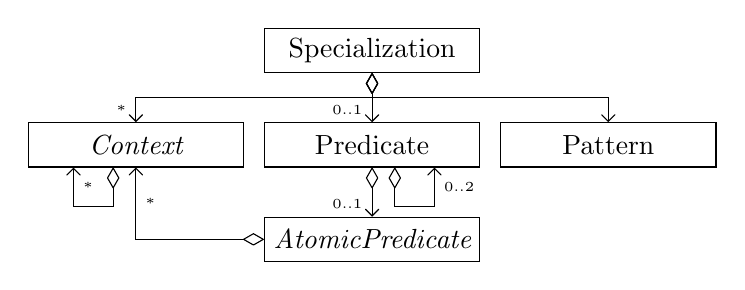
\begin{tikzpicture}[x=30mm,y=12mm]
\tikzset{CODE/.style={draw,chamfered rectangle,chamfered rectangle corners=north east,text centered,minimum height=1.6em}}
\tikzset{CLASSES/.style={draw,rectangle,text centered,minimum height=1.6em}}
\tikzset{CLASS/.style={draw,rectangle,text centered,minimum height=1.6em}}
\tikzset{MULTIPART CLASS/.style={CLASS,rectangle split,rectangle split parts=2}}

\tikzset{EXTENDS/.style={draw,-open triangle 90}}
\tikzset{ASSOCIATES/.style={draw,-angle 90}}
\tikzset{INSTANTIATES/.style={draw,dashed,-angle 90}}
\tikzset{AGGREGATES/.style={draw,open diamond-angle 90}}

\tikzset{CARDINALITY/.style={auto=right,near end,font=\tiny}}

\tikzset{DINGBATS/.style={circle,fill=white,inner sep=-0.5pt}}

\begin{scope}[text width=2.5cm]
\node[CLASS] (specialization) at (0,-1) {\lstinln{Specialization}};
\path (specialization)
  -- +(-1,-1) node[CLASS] (context) {\lstinlineabstract{Context}}
  -- +(+0,-1) node[CLASS] (expression) {\lstinln{Predicate}}
  -- +(+1,-1) node[CLASS] (pattern) {\lstinln{Pattern}};
\path (expression)
  -- +(0,-1) node[CLASS] (atomic predicate) {\lstinlineabstract{AtomicPredicate}};
\end{scope}

\path [AGGREGATES] (specialization) -- +(0,-0.5) -| (pattern);
\path [AGGREGATES] (specialization) -- +(0,-0.5) -| node[CARDINALITY] {*} (context);
\path [AGGREGATES] (specialization) -- +(0,-0.5) -| node[CARDINALITY] {0..1}  (expression);

\path [AGGREGATES] (context.-135) -- ++(0,-5mm) -| node[CARDINALITY] {*} (context.-160);

\path [AGGREGATES] (atomic predicate) -| node[CARDINALITY] {*} (context);

\path [AGGREGATES] (expression) -- node[CARDINALITY] {0..1} (atomic predicate);
\path [AGGREGATES] (expression.-45) -- ++(0,-5mm) -| node[CARDINALITY] {0..2} (expression.-20);

\end{tikzpicture}
\caption{Meta-model of a Specialization in ALIA4J.}
\label{fig:specialization}
\end{figure}

\paragraph{Plain Instance Pointcuts}
For pointcut expressions that are directly provided, we use a library function provided by ALIA4J which takes a String containing an AspectJ pointcut as input.
We have extended this library to also accept the \lstinln{returning} pointcut designator.

%\begin{lstlisting}[float,caption={Example of an instance pointcut using composition and type refinement}, label=lst:example:compo:ref,moreemph=instance]
%static instance pointcut ${ipc}<${Type}>:
%ipc1<${Type2}> || ~\label{lst:example:ip:or}~
%before(${pc_add_before}) || after(${pc_add_after}) UNTIL 
%before(${pc_remove_before}) || after(${pc_remove_after};
%\end{lstlisting}
\begin{lstlisting}[caption={Example of a plain instance pointcut}, label=lst:example:plainip,moreemph=instance]
static instance pointcut ${ipc}<${Type}>:
before(${pc_add_before}) || after(${pc_add_after}) UNTIL 
before(${pc_remove_before}) || after(${pc_remove_after};
\end{lstlisting}

For the example instance pointcut presented in listing~\ref{lst:example:plainip}, we show the code generated for the method creating the LIAM model for the add_before pointcut in listing~\ref{lst:example:compoRefGen}; the other methods are generated analogously.
Line~\ref{lst:example:simple} shows the transformation of an AspectJ pointcut into a set of Specializations in the LIAM meta-model by passing the pointcut as a String---represented by \lstinline!${pc_add_before}! in listings~\ref{lst:example:plainip} and~\ref{lst:example:compoRefGen}---to the above mentioned library function.

\begin{lstlisting}[caption={Template for creating the LIAM model for the add_before expression},label={lst:example:compoRefGen}]
private static Set<Specialization> ${ipc}_add_before;
public static Set<Specialization> ${ipc}_add_before() {
	if (${ipc}_add_before == null) {
		${ipc}_add_before = Util.toSpecializatons("${pc_add_before}", ${Type}); ~\label{lst:example:simple}~
	}
	return ${ipc}_add_before;
}
\end{lstlisting}

\paragraph{Type Refinement}
An instance pointcut can also be defined by referring to another instance pointcut whereby a type restriction for the selected instances can be defined.
A template for an instance pointcut defined as such is as follows:

\begin{lstlisting}[numbers=none, emph={instance}]
static instance pointcut ${ipc}<${Type}>: ipc1<${Type2}>;
\end{lstlisting}

For such an instance pointcut also methods are created to produce LIAM models for the four underlying pointcuts (see the template in listing~\ref{lst:example:typeRef}).
These methods first invoke the corresponding methods of the referenced instance pointcut (cf.\ line~\ref{lst:example:refer}).
Second, the type restriction is added to the Predicates of the retrieved Specializations (cf.\ line~\ref{lst:example:restriction}) with the method \lstinln{addTypeConstraint}.

\begin{lstlisting}[caption={Template for creating the LIAM model for the type-refined instance pointcut},label={lst:example:typeRef}]
public static Set<Specialization> ${ipc}_add_before() {
	...
	Set<Specialization> ipRef = ipc1_add_before(); ~\label{lst:example:refer}~
	${ipc}_add_before = Util.addTypeConstraint(ipRef, ${Type2}); ~\label{lst:example:restriction}~
	...
}
\end{lstlisting}


\paragraph{Expression Refinement} 
When defining a new instance po-intcut through expression refinement, for each of the four underlying pointcut expressions, a plain pointcut expression can be \emph{and}ed or \emph{or}ed with the an underlying pointcut expression of the referenced instance pointcut. As explained in the previous section, refinement pointcut expressions must not include a binding predicate. The referred instance pointcut expression already has a binding predicate which is carried over to be used as the binding predicate for the newly composed pointcut expression.
The template for the generated method for creating the add/before LIAM model is shown in listing~\ref{lst:example:exprRef}.
It assumes that the instance pointcut is named \lstinline!${ipc}! and it refines another instance pointcut \lstinline!${ipc1}! by \emph{and}ing the pointcut expression \lstinline!${ipc1_add_before}! to the add/before underlying pointcut.
If the pointcuts are \emph{or}ed, correspondingly the method \lstinline!orSpecializations! is used in line~\ref{lst:example:composition}.

These utility methods are provided as runtime library for the instance pointcuts.
The method \lstinline!andSpecializations! forms the conjunction of the Predicates and Patterns of the passed Specialization sets.
If \lstinline!ipRef! is empty, the conjunction is also empty and an empty set is returned.
Otherwise, the Context declared by the Specializations \lstinline!ipRef! is copied to the ones newly created by the \lstinline!andSpecializations! method.
The method \lstinline!orSpecializations! is implemented similarly.
But it forms the disjunction of Predicates and Patterns and if \lstinline!ipRef! is empty, an exception is raised.

\begin{lstlisting}[caption={Generated code for creating the LIAM model for the add/before pointcut of the instance pointcut created with expression refinement},label={lst:example:exprRef}]
public static Set<Specialization> ${ipc}_add_before() {
	...
	Set<Specialization> plainIPExpr = Util.toSpecializatons("${pc_add_before}", ${Type}); ~\label{lst:example:simple}~
	Set<Specialization> ipRef = ipc1_add_before(); ~\label{lst:example:ref}~
	${ipc}_add_before = Util.andSpecializations(ipRef, plainIPExpr); ~\label{lst:example:composition}~
	...
}
\end{lstlisting}

\paragraph{Deployment}

In each of the above cases, the created LIAM models of the pointcuts must be associated with advice invoking the add or remove method for the instance pointcut.
In a LIAM model this is achieved by defining an Attachment, which roughly corresponds to a pointcut-advice pair.
An Attachment refers to a set of Specializations, to an \emph{Action}, which specifies the advice functionality, and to a \emph{Schedule Information}, which models the time relative to a join point when the action should be executed, e.g., ``before'' the join point (cf.\ line~\ref{lst:deploy:schedule}).

Listing~\ref{lst:deployment} shows the generated code for creating and deploying the bookkeeping Attachments.
The first Attachment uses the set of Specializations returned by the \lstinline!${ipc}add_before! method (cf.\ line~\ref{lst:deploy:specializations}) and specifies the \lstinline!${ipc}_addInstance! method as action to execute at the selected join points (cf.\ line~\ref{lst:deploy:action}).
As relative execution time, the Attachment uses a ``SystemScheduleInfo''; this is provided by ALIA4J for Attachments performing maintenance whose action should be performed before or after all user actions at a join point, such that all user actions observe the same state of the maintained data.
Thus, when reaching a selected join point the instance is added to the instance pointcut's multiset before any other action can access its current content.
The other Attachments are created analogously.
In the end, all Attachments are deployed through the ALIA4J \lstinln{System} (cf.\ line~\ref{lst:deploy:deploy}).

\begin{lstlisting}[float,caption={Deployment of the bookkeeping for an instance pointcut.},label=lst:deployment]
public static void ${ipc}_deploy() {
	org.alia4j.fial.System.deploy( ~\label{lst:deploy:deploy}~
		new Attachment(
			${ipc}_add_before(), ~\label{lst:deploy:specializations}~
			createStaticAction(void.class, ${Aspect}.class, "${ipc}_addInstance", new Class[]{${Type}.class}) ~\label{lst:deploy:action}~
			SystemScheduleInfo.BEFORE_FARTHEST), ~\label{lst:deploy:schedule}~
		|Create Attachments for the other three parts analogously.|
		|For the ``after'' parts, use SystemScheduleInfo.AFTER_FARTHEST.|
		|For the ``remove'' parts, specify method ${ipc}_removeInstance.|
		);
}
\end{lstlisting}

\subsection{Composite Instance Pointcuts}

Composite instance pointcuts require a different compilation strategy because they do not have the four underlying pointcut expressions.
The data of a composite instance pointcut changes when the data of one of its referenced instance pointcuts is updated.
The corresponding events happen during the execution of the generated methods \lstinline!${ipc}_addInstance! and \lstinline!${ipc}_removeInstance!.
Therefore, a different mechanism is needed than for the non-composite instance pointcuts which depend on user events.

\paragraph{Intersection and Union}

When an instance pointcut \lstinline!${ipc}! are composed by forming the union or intersection of other instance pointcuts (\lstinline!${ipcX}!), the content of the maintained multiset potentially changes whenever an instance is added to or removed from one of the referenced instance pointcuts---events already exposed through \lstinline!${ipcX}_instanceAdded! or \newline\lstinline!${ipcX}_instanceRemoved! pointcuts.
For the maintenance of a composite instance pointcut a method is generated which reacts to the join points matching the disjunction of all these pointcuts.
The argument of this method is the instance exposed by these pointcuts, i.e., the instance that has either been added to or removed from a reference instance pointcut.
When the maintenance method is invoked, we know the cardinality of this instance potentially changes in the multiset of the instance pointcut \lstinline!${ipc}!.
The cardinality of other instances cannot change.
The generated method, therefore, re-calculates the cardinality of the affected instance and changes its value in \lstinline!${ipc}_data!.

To generate appropriate code, the compiler first builds a binary expression tree for the composition expression.
Next, it traverses this tree and generates different code for the cases that the visited node is an instance pointcut reference, or an \texttt{inter} or \texttt{union} operator.
For an instance pointcut reference, code is generated that retrieves the cardinality of the instance in the multiset of the referenced instance pointcut.
For an \texttt{inter} and \texttt{union} operator, code is generated that calculates the minimum and maximum, respectively, of both sub-expressions. Finally, the cardinality in \lstinline!${ipc}_data! is updated. 

As example, listing~\ref{lst:example:inter-union} shows the generated code for a composite instance pointcut with the set expression \lstinline!$({ipc1} union ${ipc2}) inter ${ipc3}!. Besides, the generated code remembers the old cardinality; when the cardinality changes from $0$ to $>0$ or vice versa, the generated method invokes the method \lstinline!${ipc}_instanceAdded! \lstinline!${ipc}_instanceRemoved!, respectively. 

\begin{lstlisting}[float,caption={The update method generated from a composition expression},label=lst:example:inter-union]
public static void ${ipc}_update(Object o) {
	int oldCardinality = ${ipc}_cardinality(o);
	int newCardinality =
		Math.min(
			Math.max(
				${ipc1}_cardinality(o),
				${ipc2}_cardinality(o)),
			${ipc3}_cardinality(o));
	${ipc}setCardinality(o, newCardinality);
	if (oldCardinality == 0 and newCardinality > 0)
		${ipc}_instanceAdded(o);
	else if (oldCardinality > 0 and newCardinality == 0)
		${ipc}_instanceRemoved(o);
}
\end{lstlisting}

As in the case of non-composite instance pointcuts, a LIAM Attachment is generated and deployed which associates the Specializations corresponding to the pointcuts with the generated method.

\paragraph{Type Refinement for Composite Instance Pointcuts}

Instance pointcuts which are defined by means of type refined composite instance pointcuts, are treated similar to the case above.
A method is generated which is executed when the referenced instance pointcut changes.
The method checks whether the type of the added or removed object is assignment compatible with the type restriction.
If this is the case, the same operation (adding or removing the instance) is performed on the multiset of the refining instance pointcut.

\subsection{Compiling Plain AspectJ constructs}
To ensure consistent ordering between AspectJ advice and our implementation of instance pointcuts (i.e., that our bookkeeping advice are executed before user advice), the AspectJ point\-cut-advice definitions must be processed by ALIA4J.
This is possible because ALIA4J can integrate with the standard AspectJ tooling.
Using command line arguments the AspectJ compiler can be instructed to omit the weaving phase.
The advice bodies are converted to methods and pointcut expressions are attached to them using Java's annotations which are read by the ALIA4J-AspectJ integration and transformed into Attachments at program start-up.
The code generated by our compiler consists of the above explained methods, as well as plain AspectJ definitions.
When compiling this code with the mentioned command line options, the regular AspectJ pointcut-advice and the behavior of the instance pointcuts are both executed by ALIA4J, thus ensuring a consistent execution order.



\section{Validation}
\label{sect:checking}
%\label{sect:validation}
The instance pointcuts approach satisfies the goals we have stated at the beginning of Section~\ref{sect:approach} and in Section~\ref{sect:compilation} we have shown that instance pointcuts can be compiled modularly.
Our approach provides:

\begin{itemize}
\item A concise syntax, which is used to generate the necessary book-keeping code
\item additional features to declaratively create refined sets, reusing already created instance pointcuts
\item a composition mechanism, which uses set operations, that allows modular definition of instance pointcuts.
\end{itemize}

Let us revisit the problem we have identified in section~\ref{sect:motivation} and provide an implementation that uses instance pointcuts shown in listing~\ref{lst:discountip} (this listing only includes the changed code, the rest is identical to listing~\ref{lst:discountaop}). The instance pointcut \lstinln{surpriseDiscount} successfully encapsulates the bookkeeping concern, which reduces the concern specific lines of code to a third of the AspectJ solution. The discount alert advice now uses the \lstinln{surpriseDiscount_instanceAdded} set monitoring pointcut (lines~\ref{discountip:alertb}~\textendash~\ref{discountip:alerte}). Also, in order to access the instance pointcut set, the code now uses the set access method as in line~\ref{ip:around:access}. Introducing new concerns to this code, like refining the \lstinln{surpriseDiscount} instance pointcut to select objects with prices that are higher than 50\$ (Listing~\ref{lst:exprrefine}) requires very little amount of code.

\begin{lstlisting}[float=h, moreemph=instance, caption={The instance pointcut implementation of the discount alert concern}, label={lst:discountip}]
aspect SDiscount{
	static instance pointcut surpriseDiscount<Product>: after(call(* ProductManager.submitDiscount(..)) && args(instance, SurpriseDiscount))
		UNTIL after(call(* ProductManager.withdrawDiscount(..)) && args(instance, SurpriseDiscount));
	after(Product p):surpriseDiscount_instanceAdded(p){ ~\label{discountip:alertb}~
		OnlineShop.INSTANCE().createDiscountAlert(p);
	}~\label{discountip:alerte}~
	void around(String listType):display(listType){
	...
			OnlineShop.instance().getUI()
				.display(SDiscount.surpriseDiscount()); ~\label{ip:around:access}~
	}...
}
\end{lstlisting}

A declarative syntax such as that of instance pointcuts, generally allows performing various checks, generate well-placed error or warning markers and informative warning/error messages.
In the following we discuss checks we deem useful and possible to implement based on our language.
Proving their feasibility by implementing the checks is subject to future work.

\paragraph*{Non-existent/Incompatible types} If the type declared by the instance pointcut does not exist, this is a compile error. Instance pointcuts provide an additional check during type refinement; it is a compile error if the refinement type is not a subtype of the referenced pointcut's declared type. In the Java solution the error marker is placed at the line of the \lstinln{instanceof} check, without giving any context to why the \lstinln{instanceof} check is performed. The instance pointcut error marker is placed at line of the refinement, with an elaborate error message explaining the type mistake.

Type compatibility is also an issue while composing instance pointcuts. The typing effects of the composition is previously mentioned in section~\ref{sect:compo}. If in a composite instance pointcut declaration, the instance type is explicit, then the type compatibility between the composite and the component instance pointcuts' should be checked. The compiler determines the appropriate type for every composite instance pointcut, whether the instance type is explicit or not. The computed type is then compared to the declared type; the declared type must be the same or a super type of the computed type. If there's an incompatibility, we put an error marker at the line where the type was declared, indicating the composed type is not compatible with the declared type of the composite instance pointcut.


\paragraph*{Empty Sets} The add expression of an instance pointcut is responsible for populating the instance pointcut set. If the pointcut expressions defined in the add expressions do not match any join-points then it is guaranteed that the instance pointcut set will always be empty. This case is displayed as a compile-time warning which indicates that no objects will be selected. During the expression refinement, composition of the new pointcuts and the referenced one may result in non-matching pointcut expressions.
%For instance ANDing an \lstinln{execution} pointcut to a pointcut expression that already has a \lstinln{call} pointcut will result in a pointcut expression that does not match any join-points, consequently any events.
Currently we do not perform any control-flow analysis to check for empty sets. Such a check will help us to identify cases where even if the add expression matches, no objects are added to the set.

\paragraph*{Double selection} Instance pointcut syntax allows to select the same join-point in both before and after events in the same sub-expression. In Listing~\ref{lst:objversion} such a case is illustrated. The \lstinln{Product} object is added before it is applied a discount, and once again after the discount is applied. This will increment the cardinality of the same object twice. The analogous case exists for the remove expressions. The object is removed from the set \emph{twice}. This behaviour is consistent with an instance pointcut's regular behaviour, but we still raise a separate warning for the add and remove cases to notify the developer, in case of a copy-paste error.

\begin{lstlisting}[float=h!, moreemph=instance, caption={Adding the same object before and after the same join-point}, label={lst:objversion}]
static instance pointcut surpriseDiscountDouble<Product>:
	before(call(* ProductManager.submitDiscount(..))
	&& args(instance, SurpriseDiscount))
	~$\|$~
	after(call(* ProductManager.submitDiscount(..))
	&& args(instance, SurpriseDiscount))
\end{lstlisting}

\paragraph*{Expression Refinement Checks}During expression refinement there is a special case when the refined instance pointcut is referencing a non-existent event selector and the $\|$ boolean operator is used.  Assume that \lstinln{ipc1} only has an \lstinln{add_before} expression. While refining this instance pointcut the developer mistakenly writes the following:

\begin{lstlisting}
ipc2<T>: add_before:ipc1.add_before
	add_after: ipc1.add_after ~$\|$~ call(..);
\end{lstlisting}

This definition refers to the non-existent \lstinln{add_after} expression. This is a compile error since, while the \lstinln{call} pointcut is selecting joinpoints, no objects are bound.  This is illegal to have in an instance pointcut expression. Note that if the operation was \&\& there would be no compile error since, the \lstinln{add_after} expression of \lstinln{ipc2} would simply be empty and \lstinln{ip2}'s add expression would only comprise of \lstinln{ipc1}'s \lstinln{add_before} event selector.



\section{Related Work}
AO-extensions for improving aspect-object relationships are proposed in several studies. Sakurai et al.~\cite{sakurai2004association} proposed Association Aspects. This is an extension to aspect instantiation mechanisms in AspectJ to declaratively associate an aspect to a tuple of objects. In this work the type of object tuples are declared with a \lstinln{perobjects} clause and the specific objects are selected by pointcuts. This work offers a method for defining relationships between objects. Similar to association aspects, Relationship Aspects \cite{pearce2006relationship} also offer a declarative mechanism to define relationships between objects, which are cross-cutting to the OO-implementation. This work focuses on managing relationships between associated objects. Bodden et al.~\cite{bodden2008relational} claim that the two above approaches lack generality and propose a tracematch-based approach. Although the semantics of the approaches are very similar, Bodden et al.\ combine features of thread safety, memory safety, per-association state and binding of primitive values or values of non-weavable classes. Our approach, also extending AO, differs from these approaches since our aim is not defining new relationships but using the existing structures as a base to group objects together for behaviour extensions. Our approach also offers additional features of composition and refinement.

The ``dflow'' pointcut~\cite{kawauchi:aosd-aosdsec04} is an extension to AspectJ that can be used to reason about the values bound by pointcut expressions. Thereby it can be specified that a pointcut only matches at a join point when the origin of the specified value from the context of this join point did or did not appear in the context of another, previous join point (also specified in terms of a pointcut expression). This construct is limited to restricting the applicability of pointcut expressions rather than reifying all objects that match certain criteria, as our approach does.

Another related field is Object Query Languages~(OQL) which are used to query objects in an object-oriented program (e.g.,~\cite{cluet1998designing}). However OQLs do not support event based querying, which selects objects based on the events they participate in, as presented in our approach. It is interesting to combine instance pointcuts with OQL. For example instance pointcuts can be used as a predicate in OQL expressions, in order to select from phase-specific object sets. We will explore possible applications in future work.

Type States~\cite{DeLine2004} allow to define a state chart for a type.
This specifies which states an object of that type can be in and what causes state transitions.
Similar to our approach, state transitions are triggered by runtime events.
However unlike instance pointcuts, in type states an objects state can only change at method calls where the object is the receiver; with instance pointcuts, objects life-cycle phases can be defined more flexibly by referring to any event where the object is in the dynamic context, e.g., passed as argument or result value.
The purpose of the type states approach is to facilitate more powerful invariant checking at compile-time, whereas we provide a mechanism to actually track object sets at runtime.
It would be interesting to investigate possibilities for combining both approaches in the future.

\section{Conclusion and Future Work}
In this work we have presented instance pointcuts, a specialized pointcut mechanism for reifying phase-specific object sets.
Our approach provides a declarative syntax for defining events when an object starts or ends to belong to a life-cycle phase.
Instance pointcuts maintain multisets providing a count for objects which enter the same life-cycle phase more than once.
Instance pointcut sets can be accessed easily and any changes to these sets can also be monitored with the help of automatically created set monitoring pointcuts.
The sets can be declaratively composed, which allows reuse of existing instance pointcuts and consistency among corresponding multisets.
Finally, we have presented our modular compilation approach for instance pointcuts based on AspectJ and the ALIA4J Language implementation architecture.
ALIA4J provided us with the flexibility AspectJ lacked in instance pointcut composition and type refinement.

The syntax and expressiveness of instance pointcuts partially depend on the underlying AO language;
this is evident especially in our usage of the AspectJ pointcut language in the specification of events.
Since AspectJ's join points are ``regions in time'' rather than events, we had to add the ``before'' and ``after'' keywords to our add and remove expressions.
Thus, compiling to a different target language with native support for events (e.g., EScala~\cite{Gasiunas2011} or Composition Filters~\cite{Bergmans2001b}, the point-in-time join point model~\cite{masuharafine}) would influence the notation of these expressions.

We think the instance pointcut concept is very flexible and can be useful in various applications.
It eliminates boilerplate code to a great extent and provides a readable syntax.
We believe that the reuse and composition mechanisms offered by instance pointcuts are beneficial for software evolution since they make it easy to create tailored variations according to new requirements.



One relevant field of application for instance pointcuts are design patterns which are known to be good examples for aspect-oriented programming~\cite{hannemann:oopsla02}.
Many design patterns exist for defining the behaviour for groups of objects; thus implementing them with our instance pointcuts seems to provide a natural benefit.
We are currently working on creating object adapters wrapping the objects reified by an instance pointcut.


\bibliographystyle{abbrv}
\bibliography{biblio}
\end{document}


